\documentclass{article}
\usepackage{amsfonts, amsmath, amssymb, amsthm} % Math notations imported
\usepackage{enumitem}
\usepackage{graphicx}
\usepackage[margin=1in]{geometry}
\usepackage{setspace}
\graphicspath{{./images/}} % Path to images

% \begin{figure}[htb!]
%      \centering
%      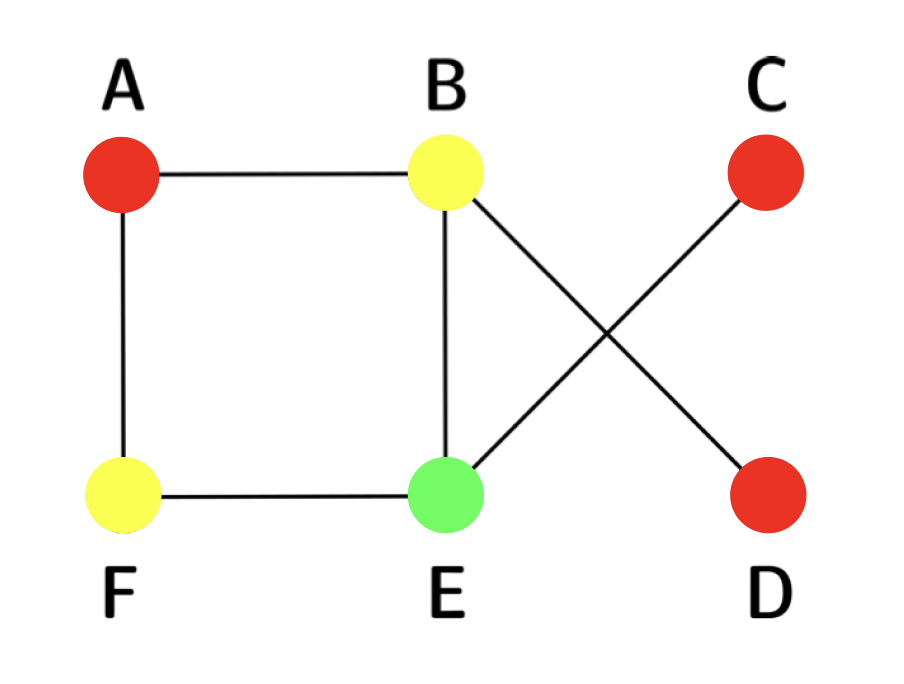
\includegraphics[scale=0.5]{coloring.png}
%      \caption{Coloring of the graph.}
% \end{figure}

\newtheorem{thm}{Theorem}
\newtheorem{proposition}[thm]{Proposition}
\newtheorem{cor}[thm]{Corollary}

% title information
\title{Math 104 HW1}
\author{Neo Lee}
\date{09/01/2023}

\setstretch{1.15}
% main content
\begin{document} 

% placing title information; comment out if using fancyhdr
\maketitle 

\section*{Exercise 1.3}
\begin{proposition}
    $1^3 + 2^3 + \cdots + n^3 = (1+2+\cdots + n)^2$ for all positive integers $n$.
\end{proposition}    
\begin{proof}
    We proceed by induction.

    \underline{Base case}: $n=1$. We have $1^3 = 1^2$.

    \underline{Inductive step}: Assume that $1^3 + 2^3 + \cdots + k^3 = (1+2+\cdots +k)^2$ for 
    some $k \in \mathbb{N}$. Now consider $k+1$,
    \begin{align*}
        1^3 + 2^3 + \cdots + k^3 + (k+1)^3 & = (1+2+\cdots +k)^2 + (k+1)^3 \\
        & = \left(\frac{(k+1)\cdot k}{2}\right)^2 + (k+1)^3 \\ 
        & = \frac{(k+1)^2\cdot k^2 + (k+1)^2 \cdot 4(k+1)}{4} \\
        & = \frac{(k+1)^2(k^2 + 4k + 4)}{4} \\
        & = \frac{(k+1)^2(k+2)^2}{4} \\
        & = \left(\frac{(k+1)\cdot (k+2)}{2}\right)^2 \\
        & = (1+2+\cdots +(k+1))^2.
    \end{align*}

    Hence, by the principle of mathematical induction, $1^3 + 2^3 + \cdots + n^3 = 
    (1+2+\cdots + n)^2$ for all positive integers $n$.
\end{proof}
\bigbreak

\section*{Exercise 1.5}
\begin{proposition}
    $1 + \frac{1}{2} + \frac{1}{4} + \cdots + \frac{1}{2^n} = 2 - \frac{1}{2^n}$ for all positive 
    integers $n$.
\end{proposition}
\begin{proof}
    We again proceed by induction.

    \underline{Base case}: $n=1$. We have $1 + \frac{1}{2} = 2 - \frac{1}{2}$.

    \underline{Inductive step}: Assume that $1 + \frac{1}{2} + \frac{1}{4} + \cdots 
    + \frac{1}{2^k} = 2 - \frac{1}{2^k}$ for some $k \in \mathbb{N}$. Now consider $k+1$,
    \begin{align*}
        1 + \frac{1}{2} + \frac{1}{4} + \cdots + \frac{1}{2^k} + \frac{1}{2^{k+1}} & = 
        2 - \frac{1}{2^k} + \frac{1}{2^{k+1}} \\
        & = 2 - \frac{1}{2^k} + \frac{1}{2^k}\cdot \frac{1}{2} \\
        & = 2 - \frac{1}{2^k}\left(1 - \frac{1}{2}\right) \\
        & = 2 - \frac{1}{2^k}\cdot \frac{1}{2} \\
        & = 2 - \frac{1}{2^{k+1}}.
    \end{align*}

    Hence, by the principle of mathematical induction, $1 + \frac{1}{2} + \frac{1}{4} + \cdots
    + \frac{1}{2^n} = 2 - \frac{1}{2^n}$ for all positive integers $n$.
\end{proof}
\bigbreak

\section*{Exercise 1.11}
\begin{enumerate}[label=(\alph*)]
    \item \begin{proposition}
        If $n^2 + 5n + 1$ is an even integer, then $(n+1)^2 + 5(n+1) + 1$ is also an even integer 
        for $n \in \mathbb{N}$.
    \end{proposition}

    Consider 
    \begin{align*}
        (n+1)^2 + 5(n+1) + 1 & = n^2 + 2n + 1 + 5n + 5 + 1 \\
        & = n^2 + 5n + 1 + 2n + 6 \\
        & = (n^2 + 5n + 1) + 2(n+3) \\
        & = 2k + 2(n+3) \qquad (\emph{for some } k \in \mathbb{Z} \because \emph{$n^2 + 5n + 1$ is 
        an even integer}) \\
        & = 2(k + n + 3).
    \end{align*}
    Hence, $(n+1)^2 + 5(n+1) + 1$ is an even integer.

    \item For which $n \in \mathbb{N}$ is $n^2 + 5n + 1$ an even integer?
    \begin{proof}[Solution]
        If $n$ is even, then $n^2 + 5n + 1 = (2k)^2 + 5(2k) + 1 = 2(2k^2 + 5k) + 1$ for some $k \in 
        \mathbb{Z}$, thus is an odd integer. If $n$ is odd, then $n^2 + 5n + 1 = (2j+1)^2 + 5(2j+1)
        + 1 = 2(2j^2 + 7j + 3) + 1$ for some $j \in \mathbb{Z}$, thus is also an odd integer. 
        Hence, $n^2 + 5n + 1$ is never an even integer.

        The moral of the exercise is that even the inductive step is true, the proposition is not
        necessarily true without a proper and true base case.
    \end{proof}
\end{enumerate}
\bigbreak

\section*{Exercise 2.7}
\begin{enumerate}[label=(\alph*)]
    \item \begin{proposition}
        $\sqrt{4+2\sqrt{3}} - \sqrt{3}$ is rational.
    \end{proposition}

    \begin{proof}
        Let $x = \sqrt{4+2\sqrt{3}} - \sqrt{3}$. Now, evaluate
        \begin{align*}
            x & = \sqrt{4+2\sqrt{3}} - \sqrt{3} \\
            (x + \sqrt{3})^2 & = 4 + 2\sqrt{3} \\
            x^2 + 2x\sqrt{3} + 3 & = 4 + 2\sqrt{3} \\
            x^2 - 1 & = \sqrt{3}(2-2x) \\
            (x^2 - 1)^2 & = 3(2-2x)^2 \\
            x^4 - 2x^2 + 1 & = 12 - 24x + 12x^2 \\
            x^4 - 14x^2 + 24x - 11 & = 0.
        \end{align*}

        By the rational zeros theorem, the only possible rational roots are $\pm 1, \pm 11$. Indeed, 
        $x = 1$ is a root of the equation, and 1 is obviously rational.
    \end{proof}

    \item \begin{proposition}
        $\sqrt{6 + 4\sqrt{2}} - \sqrt{2}$ is rational.
    \end{proposition}

    \begin{proof}
        Again, let $x = \sqrt{6 + 4\sqrt{2}} - \sqrt{2}$. Now, evaluate
        \begin{align*}
            x & = \sqrt{6 + 4\sqrt{2}} - \sqrt{2} \\
            (x + \sqrt{2})^2 & = 6 + 4\sqrt{2} \\
            x^2 + 2x\sqrt{2} + 2 & = 6 + 4\sqrt{2} \\
            x^2 - 4 & = \sqrt{2}(4-2x) \\
            (x^2 - 4)^2 & = 2(4-2x)^2 \\
            x^4 - 8x^2 + 16 & = 32 - 32x + 8x^2 \\
            x^4 - 16x^2 + 32x - 16 & = 0.
        \end{align*}

        By the rational zeros theorem, the only possible rational roots are $\pm 1, \pm 2, \pm 4,
        \pm 8, \pm 16$. Indeed, $x = 2$ is a root of the equation, and 2 is obviously rational.
    \end{proof}
\end{enumerate}
\bigbreak

\section*{Exercise 2.8}
Find all rational solutions of the equation $x^8 - 4x^5 + 13x^3 - 7x + 1 =0$.

\begin{proof}[Solution]
    By rational zeros theorem, the only possible rational candidates to the equation is only 
    $\pm 1$. Only -1 satisfies the equation, thus -1 is the only rational solution.
\end{proof}
\bigbreak

\section*{Exercise 3.1}
    \begin{enumerate}[label=(\alph*)]
        \item Which of the ordered field properties A1-A4, M1-M4, DL, O1-05 fail for $\mathbb{N}$.
        \begin{proof}[Solution]
            A3: $\mathbb{N}$ does not have additive identity. \\
            A4: $\mathbb{N}$ does not have additive inverse. \\
            M4: $\mathbb{N}$ does not have multiplicative inverse. 
        \end{proof}

        \item Which of the ordered field properties A1-A4, M1-M4, DL, O1-05 fail for $\mathbb{Z}$.
        \begin{proof}[Solution]
            M4: $\mathbb{Z}$ does not have multiplicative inverse.
        \end{proof}
    \end{enumerate}
\bigbreak

\section*{Exercise 3.6a}
\begin{proposition}
    $|a+b+c|\le |a|+|b|+|c|$ for all $a,c,b \in \mathbb{R}$.
\end{proposition}
\begin{proof}
    \begin{align*}
        |a+b+c| & = |(a+b)+c| \\
        & \le |a+b| + |c| \qquad (\emph{triangle inequality on } (a +b), c) \\
        & \le |a| + |b| + |c|. \qquad (\emph{triangle inequality on } a, b)
    \end{align*}
\end{proof}
\end{document}
